\section{Experimento 1 - Medición de la impedancia de un inductor mediante una onda de
corriente triangular}
Para llevar a cabo este experimento se utilizó el siguiente transformador que se encuentra disponible en el pañol:
\begin{figure}[H]
    \centering
    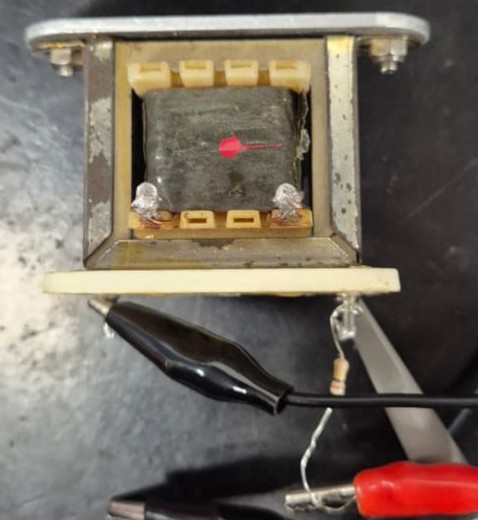
\includegraphics[width=0.5\textwidth]{images/transformador.jpeg}
    \caption{Transformador utilizado en el experimento.}
\end{figure}
El cual tiene una resistencia serie nominal de 200 $\Omega$ y una inductancia nominal de 15H:
\begin{figure}[H]
    \centering
    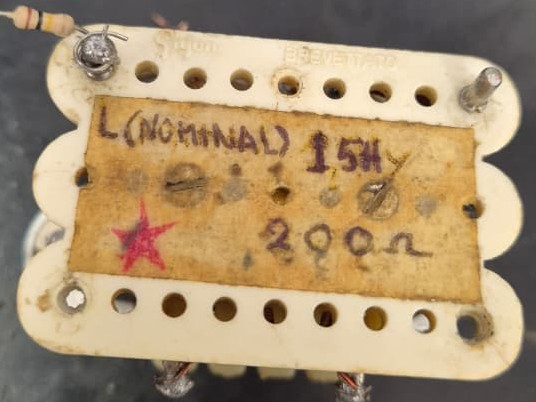
\includegraphics[width=0.5\textwidth]{images/transformador1.jpeg}
    \caption{Valores nominales del transformador utilizado en el experimento.}
\end{figure}
Para el experimento se conectaron los instrumentos de la siguiente manera:
\begin{figure}[H]
    \centering
    
\includegraphics[width=0.5\textwidth]{images/esquema1.png}
    \caption{Esquema de medición}
\end{figure}
Como la bobina tiene perdidas se modela como una ideal con una resistencia en serie que representa sus perdidas, por lo que la tensión de salida que se observa en C1 es la suma de estas dos tensiones "$e_{L}$" y "$e_{R}$". La bobina actúa como un derivador, por lo que al inyectarla una señal triangular la salida del circuito será una onda cuadrada "$e_{L}$" la cual tiene una pendiente que es generada por la tensión de la resistencia "$e_{R}$", ya que esta copia la forma de la señal. Como este actúa como un derivador, cualquier ruido de alta frecuencia será amplificado ensanchando a la onda cuadrada.
\begin{figure}[H]
    \centering
    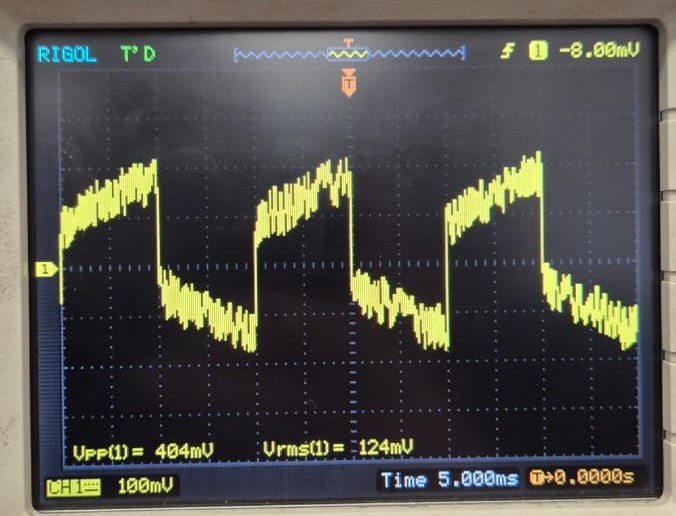
\includegraphics[width=0.5\textwidth]{images/ondacuadrada1.jpeg}
    \caption{Señal de salida del circuito.}
\end{figure}
La entrada es una señal triangular de $20Vpp$ en serie con la resistencia r de alto valor para que forme una fuente de corriente constante. Para poder medir los valores de $e_{L}$ y de $e_{R}$ como se muestra en la figura  \ref{fig:medi1} se utilizó el tipo de muestra promedio para poder obtener un valor más estable de la señal.
\begin{figure}[H]
    \centering
    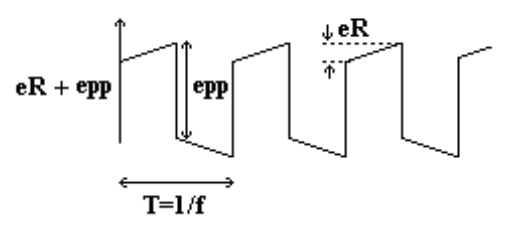
\includegraphics[width=0.5\textwidth]{images/esquemamedicion.png}
    \caption{Esquema de medición de $e_{L}$ y $e_{R}$.}
    \label{fig:medi1}
\end{figure}

\begin{table}[htbp]
    \centering
    \caption{Registro de mediciones del Experimento 1}
    \label{tab:mediciones_exp1}
    % Aumenta la altura de las filas para que sea más legible
    \renewcommand{\arraystretch}{1.3} 
    % \columnwidth hace que ocupe exacto el ancho de la columna actual
    % @{\extracolsep{\fill}} distribuye el espacio sobrante equitativamente
    \begin{tabular*}{\columnwidth}{@{\extracolsep{\fill}}|c|c|c|c|}
        \hline
        f & f1: 50 Hz & f2: 100 Hz & f3: 200 Hz \\ \hline
        r & 100 k$\Omega$ & 100 k$\Omega$ & 100 k$\Omega$ \\ \hline
        I (mA) & 57$\mu A$ & 57$\mu A$ & 57$\mu A$ \\ \hline
        epp=2.eL & 224mV & 444mV & 488mV \\ \hline
        eR & 80mV & 108mV & 88mV \\ \hline
        L & 19,6H & 19,47H & 10,7H \\ \hline
        R & 1403 $\Omega$ & 1894,75 $\Omega$ & 1543,86 $\Omega$ \\ \hline
    \end{tabular*}
\end{table}
Las expresiones utilizadas para calcular la inductancia y la resistencia de la bobina fueron las siguientes:
\begin{equation}
    L = \frac{e_{pp}}{4 \cdot I \cdot f}
\end{equation}
\begin{equation}
    R = \frac{e_{R}}{I}
\end{equation}
Las siguientes imagenes muestran la forma de onda de la señal de salida en dos de las frecuencias utilizadas en el experimento, 50Hz y 200Hz.
\begin{figure}[H]
    \centering
    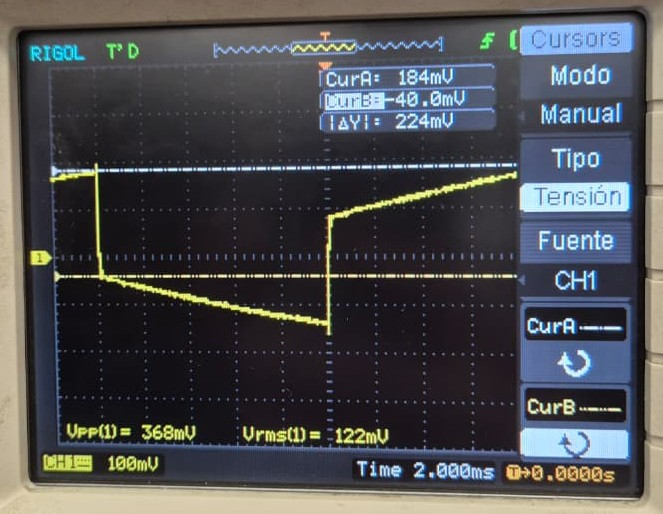
\includegraphics[width=0.5\textwidth]{images/epp50.jpeg}
    \caption{Medición de $e_{pp}$ a 50Hz.}
\end{figure}
\begin{figure}[H]
    \centering
    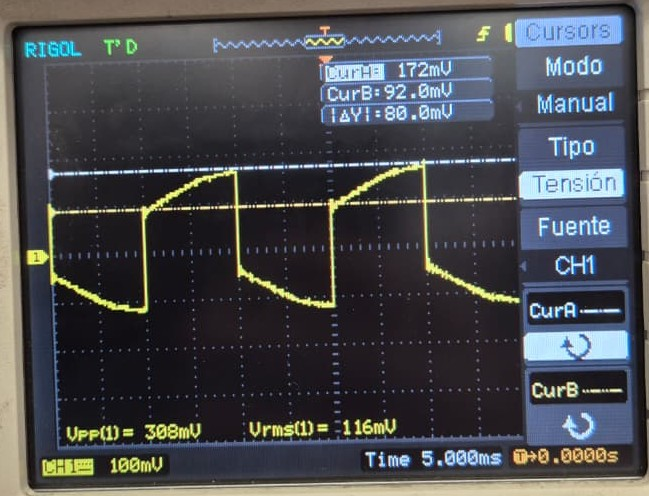
\includegraphics[width=0.5\textwidth]{images/er50.jpeg}
    \caption{Medición de $e_{R}$ a 50Hz.}
\end{figure}
\begin{figure}[H]
    \centering
    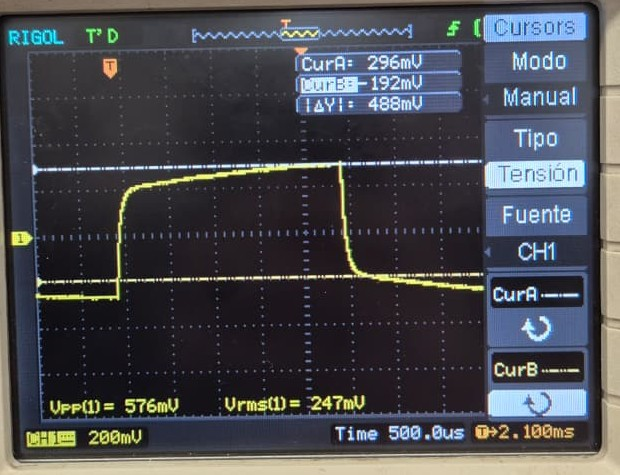
\includegraphics[width=0.5\textwidth]{images/epp200.jpeg}
    \caption{Medición de $e_{pp}$ a 200Hz.}
\end{figure}
\begin{figure}[H]
    \centering
    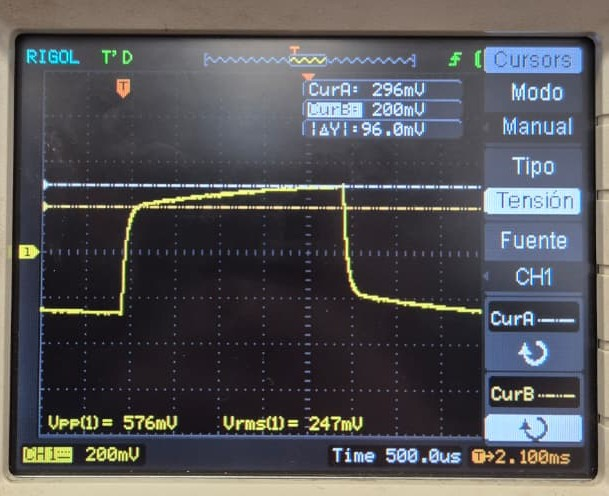
\includegraphics[width=0.5\textwidth]{images/er200.jpeg}
    \caption{Medición de $e_{R}$ a 200Hz.}
\end{figure}

Para el valor de (L) definitivo se calcula la mediana de los
valores obtenidos por lo que $$L_{mediana} = 19,47H$$.
